% TEMPLATE for Usenix papers, specifically to meet requirements of
%  USENIX '05
% originally a template for producing IEEE-format articles using LaTeX.
%   written by Matthew Ward, CS Department, Worcester Polytechnic Institute.
% adapted by David Beazley for his excellent SWIG paper in Proceedings,
%   Tcl 96
% turned into a smartass generic template by De Clarke, with thanks to
%   both the above pioneers
% use at your own risk.  Complaints to /dev/null.
% make it two column with no page numbering, default is 10 point

% Munged by Fred Douglis <douglis@research.att.com> 10/97 to separate
% the .sty file from the LaTeX source template, so that people can
% more easily include the .sty file into an existing document.  Also
% changed to more closely follow the style guidelines as represented
% by the Word sample file. 

% Note that since 2010, USENIX does not require endnotes. If you want
% foot of page notes, don't include the endnotes package in the 
% usepackage command, below.

\documentclass[letterpaper,twocolumn,10pt]{article}
\usepackage{custom}
\usepackage{usenix,epsfig,endnotes,hyperref}
\usepackage{color, enumitem}
\usepackage{cleveref, float, graphicx, longtable, subcaption}

\begin{document}

%don't want date printed
\date{}

%make title bold and 14 pt font (Latex default is non-bold, 16 pt)
\title{\Large \bf Detection and Analysis of Disaster-Related Tweets}

\author{
{\rm Daniel Solomon}\\
\texttt{solomond@mail.tau.ac.il}
\and
{\rm Gal Ron}\\
\texttt{galr1@mail.tau.ac.il‬}
\and
{\rm Omri Ben-Horin}\\
\texttt{omribenhorin@mail.tau.ac.il}
}

\maketitle

% Use the following at camera-ready time to suppress page numbers.
% Comment it out when you first submit the paper for review.
\thispagestyle{empty}


\abstract{}

\begin{center}
	\parbox{200pt}{
		\todo{bla bla bla bla bla bla bla bla bla bla bla bla bla bla bla bla bla bla bla bla bla bla bla bla bla bla bla bla bla bla bla bla bla bla bla bla bla bla bla bla bla bla bla bla bla bla bla bla bla bla bla bla bla bla bla bla bla bla bla bla bla bla bla bla bla bla bla bla bla bla bla bla bla bla bla bla bla bla bla bla bla bla bla bla bla bla bla bla bla bla bla bla bla bla bla bla bla bla bla bla bla bla bla bla bla bla bla bla.}
	}
\end{center}

%%%%%%%%%%%%%%%%%%%%%%%%%%%%%%%%%%%%%%%%%%
\section{Introduction}
The popular microblogging service Twitter is a fruitful source of user-created content. With hundreds of millions of new tweets every day, Twitter has become a probe to human behavior and opinions from around the globe. The Twitter 'corpus' reflects political and social trends, popular culture, global and local happenings, and more. In addition, tweets are easy to access and aggregate in real-time. Therefore, we experience an increased interest in natural language processing research of Twitter data.

As one of the world's most widely used social networks, Twitter is an effective channel of communication and plays an important role during a crisis or emergency. The live stream of tweets can be used to identify reports and calls for help in emergency situations, such as accidents, violent crimes, natural disasters and terror attacks (which we all refer to as 'disasters' in this paper).

In this work we utilize techniques from the natural language processing pipeline (tokenization, part-of-speech tagging and named-entity recognition) to work on Twitter data, as opposed to traditional corpora, in order to detect and analyze disaster-related tweets.

\paragraph{The Dataset}
We present our experiments on a \href{https://www.crowdflower.com/data-for-everyone/}{dataset} of 10,877 tweets\endnote{\textbf{"Disasters on social media" Dataset by CrowdFlower}: Contributors looked at over 10,000 tweets culled with a variety of searches like "ablaze", "quarantine", and "pandemonium", then noted whether the tweet referred to a disaster. \url{https://www.crowdflower.com/wp-content/uploads/2016/03/socialmedia-disaster-tweets-DFE.csv}}, labeled to \textit{'disaster-related'} and \textit{'not disaster-related'} with confidence in the range $[0,1]$. For example, the following tweet is \textit{'disaster-related'} with confidence 1,

\begin{center}
	\parbox{190pt}{\tweet{Thunderstorms with little rain expected in Central California. High fire danger. \#weather \#cawx http://t.co/A5GNzbuSqq}}
\end{center}


while the following tweet is \textit{'not disaster-related'} with confidence 0.59,

\begin{center}
	\parbox{190pt}{\tweet{It's been raining since you left me // Now I'm drowning in the flood // You see I've always been a fighter // But without you I give up}}
\end{center}

Even for one who is not familiar with the Bon Jovi lyrics in the latter tweet, it is clear that the tweet does not refer to a real natural disaster. However, this observation is hard to make examining only the vocabulary used; the latter tweet contains a variety of 'disastrous' words  (e.g. \tweet{raining, drowning, flood, fighter}). This example hints that in order to reach meaningful results we may have to examine additional linguistic features of colloquial writing,  as well as Twitter-specific features such as hashtags (\tweet{\textbf{\#}}), user at-mentions (\tweet{\textbf{@}}), internet links and emoticons.


\paragraph{Our Contribution}

In this paper we present our work tackling three missions involving disaster-related tweets.

The first mission is \textit{identification} of disaster-related tweets among a variety of tweets. We implemented several classifiers, the best of which achieved \todo{\%} accuracy on the dataset. We note that this method could have easily been adjusted to identify tweets related to themes other than disasters (e.g. politics-related, sports-related, etc.), given the appropriate dataset.

The second mission is binary classification of disaster-related tweets to one of two categories, \textit{subjective tweets} (i.e. tweets that express an emotion) vs. \textit{objective tweets} (such as news reports on disasters). To achieve this we manually tagged 2,410 disaster-related tweets. The motivation behind this task is that objective tweets like informative news reports are likely to be published after the event had already become clear to emergency services, while subjective tweets may contain invaluable first-person testimonies of ongoing events.

Finally, we extracted named entities to enrich our knowledge on the disaster (mostly location)... \todo{Omri - short description of method and achievements}.

To demonstrate our framework we aggregated recent tweets from various locations in the US, extracted disaster-related tweets using our classifier, and then used named-entity recognition to discover entities related to ongoing disasters. For example, "\tweet{Hurricane Harvey}" appeared as a top named-entity among recent tweets sent from Houston, TX, which we identified as \textit{disaster-related}.

The code of our project is available at \url{https://github.com/glrn/nlp-disaster-analysis}.

\subsection{Twitter vs. Traditional Corpora}

Tweets are limited to 140 characters and are widely used by non-professional writers. Therefore, Tweet datasets have some unique features that differ from traditional corpora (such as WSJ corpus). These features should be addressed when implementing natural language processing techniques.

First, the grammar of tweets is quite different from edited news text. It is common that tweets are written as colloquial sentences in first person where the subject ('I') is omitted, as in: '\tweet{see the flames from my window OMG}'.

Tweets are also characterized by extensive use of abbreviations and slang specific to social-media (e.g. \tweet{ily} for 'I love you', \tweet{iono} for 'I don't know). Such abbreviations may squash several parts-of-speech into one token, which poses a challenge to POS tagging.

In addition, due to the colloquial nature of user-created content, it is common that proper words are replaced by phonetically or morphologically similar ones (e.g. 'wtchng' instead of 'watching', 'gr8' instead of 'great'). Users may also use capitalization irregularities, deliberate spelling errors, punctuation irregularities and interjections as a means to express their sentiment, as in the following tweet:

\begin{center}
	\parbox{190pt}{\tweet{Haha South Tampa is getting flooded hah- WAIT A SECOND I LIVE IN SOUTH TAMPA WHAT AM I GONNA DO WHAT AM I GONNA DO FVCK \#flooding}}
\end{center}

Lastly, tweets may contain a variety of tokens seen mainly in Twitter and other social media, such as: URLs; emoticons; Twitter hashtags, of the form \tweet{\#tagname}, which the authoer may supply to label a tweet; Twitter at-mentions of the form \tweet{@user} which link to other Twitter users; and Twitter discourse functions such as \tweet{RT} ("re-tweet"), indicating that a tweet was originally posted by some other Twitter user, or ellipsis dots (\tweet{...}) at the end (or beginning) of a tweet, indicating that the tweet will be continued in a subsequent tweet by the same user. We note that hashtags and at-mentions can also serve as words or phrases within a tweet, as in:

\begin{center}
	\parbox{190pt}{\tweet{Heard about the \#earthquake, stay safe everyone.}}
\end{center}

Regarding URLs, all links posted in tweets are shortened using Twitter's link service, \url{http://t.co}, and are converted to a seemingly random 23 characters URL that redirects to the original web address.


%%%%%%%%%%%%%%%%%%%%%%%%%%%%%%%%%%%%%%%%%%
\section{Analysis Wokrflow}

\paragraph{keywords} TODO

\begin{itemize}[noitemsep,nolistsep]
	\item A
	\item B
	\item C
\end{itemize}

\todo{(Gal) Complete this section}


%%%%%%%%%%%%%%%%%%%%%%%%%%%%%%%%%%%%%%%%%%
\section{Classification of Disaster-Related Tweets}

In the first part of our work we developed a classifier that identifies \textit{disaster-related} tweets from \textit{not disaster-related} tweets,  trained on a dataset of 10,877 labeled tweets. We used only tweets with label confidence $>0.9$, which is about half of the original dataset. We experimented with a Naive Bayes (NB), random forest (RF) and support vector machine (SVM) classifiers.

\paragraph{Naive Bayes}
A supervised probabilistic learning method that classify according to \textit{maximum a posteriori}. In this method we used \textit{unigram} and \textit{bigram} features.

\paragraph{Random Forest}
An ensemble learning method that uses some estimators (trees) to classify. In this method we used \textit{unigram} and \textit{bigram} features.

\paragraph{Support Vector Machine (SVM)}
A discriminative learning method that attempts to find the hyperplane that gives maximum margin between positive and negative classification on the training data, using penalty method for mistakes. In this method we used \textit{unigram}, \textit{bigram}, \textit{tweets metadata} and \textit{POS tagging} features.

\subsection{Feature Extraction}

To train the classifiers we extracted several features for each tweet:

\begin{itemize}[noitemsep]
	\item \textbf{Unigrams and bigrams} of tokens in tweet; we used a Python version of \texttt{Twokenizer}, tokenizer for Twitter data (Gimpel et al. \cite{POS-Tagging}, Myle Ott, 2013 \cite{ark-twokenize-py}).
	\item \textbf{Tweet metadata}; hashtags, at-mentions and URLs; we parsed the tweet, crawled URLs and used the referred webpage title as supplementary information.
	\item \textbf{Part-of-speech (POS) tags} (bigram and unigram); we used a twitter-specific tagset and tagger presented by Gimpel et al. \cite{POS-Tagging}.
\end{itemize}

\paragraph{Tokenization}
Splitting a tweet to tokens (separated ordered words) is hard due to irregular punctuation patterns and use of punctuation marks for emoticons. For example, the correct tokenization of '\tweet{hello (\#hashtag)}' is to the four tokens [\tweet{ hello , ( , \#hashtag , ) }], but '\tweet{hello (:}' should be split only to the tuple [ \tweet{hello , (:} ].

\texttt{Twokenizer} is a tokenizer designed for Twitter text in English that addresses these issues. It was originally developed in Python by O'Connor et al., 2010 \cite{TweetMotif}, then improved and ported to Java by Gimpel et al., 2011 \cite{POS-Tagging} and later ported back to Python \cite{ark-twokenize-py}. We use the last version by Myle Ott.

\paragraph{Metadata Extraction}
The hashtags, at-mentions, URLs and emoticons in a tweet carry information that may help better understand the subject and context. Therefore, for each tweet we created a vector of the following metadata features, which we found to be the most expressive:

\begin{itemize}[noitemsep, nolistsep]
	\item Does the tweet contain any links, and if so how many?
	\item Is '\texttt{https://twitter.com}' one of the links (i.e. a link that refers to another tweet)?
	\item Does the tweet contain a user at-mention (\tweet{@})?
	\item Does the tweet contain any hashtags (\tweet{\#}), and if so how many?
	\item Does the tweet contain a happy emoticon (e.g. \tweet{:D})?
\end{itemize}

In addition to these features, we extracted information from hashtags and URLs. We attempted to split hashtgs to separate words
looking for a CamelCase pattern (for example, \tweet{\#JeSuisCharlie} $\rightarrow$ 'Je Suis Charlie') or words separated by underline. We note that this method is not exhaustive since Twitter users tend to create hashtags composed of joined words, all lower-case.

We also found that the domain name of the URLs in a tweet may give an indication to whether the tweet is disaster-related or not (for example, a link to \texttt{https://9gag.com} is a negative hint). However, Twitter applies URL shortening on links, so for each shortened link in the dataset we attempted to reach the original Internet address. We also collected the HTML page title, which often contains the title of an article (for example, in news sites). We managed to expand 4,823 URLs out of 6,157 in the dataset.

For each tweet in the dataset we created an \textit{'extended' version} where (1) hashtags are extracted, (2) URLs are expanded to original URL followed by the page title and (3) every user at-mention is replaced by the token \_\_USERREF\_\_.
For example, the following is a tweet,

\begin{center}
	\parbox{190pt}{\tweet{http://t.co/c1H7JECFrV @RoyalCarribean do your passengers know about the mass murder that takes place in the \#FaroeIslands every year?}}
\end{center}

and its \textit{extended version} is,

\begin{center}
	\parbox{190pt}{\tweet{https://www.royalcaribbean.co.uk/ 
				Holiday Destinations - Cruise Destinations | Royal Caribbean UK.
				\_\_USERREF\_\_  do your passengers know about the mass murder that takes place in the Faroe Islands every year?
	}}
\end{center}

\paragraph{Twitter POS Tagging}
\todo{Gal \cite{POS-Tagging}}

\subsection{Results}
Dataset was divided into train (90\%) and test (10\%) sets. Each classification method was tested with \textit{unigram} features and \textit{bigram} features separately, for the \textit{SVM} classifier, \textit{tweets metadata} and \textit{POS tagging} features were tested as well. \\
Accuracy was calculated by 3 measures:
\paragraph{Total Accuracy} number of right classifications out of the total queries ($ \frac{TP + TN}{TP + FP + TN + FN } $).
\paragraph{Positive Predictive Value} number of right positive classifications out of total positive classifications ($ \frac{TP}{TP + FP} $).
\paragraph{Negative Predictive Value} number of right negative classifications out of total negative classifications ($ \frac{TN}{TN + FN} $).
\\\\
For both \textit{Random Forest} and \textit{SVM} classifiers we have tuned parameters using \textit{grid search}. For \textit{Random Forest} we have tuned the number of estimators and for \textit{SVM} we have tuned the penalty constant. \\
\paragraph{Random Forest} For the \textit{Random Forest} results \ref{fig:disaster_classification_rf}, we can observe easily that the \textit{Unigram} features have better accuracy and better \textit{NPV}, while \textit{Bigram} features have better \textit{PPV} for any number of estimators. In addition, best result for total accuracy, \textit{PPV}, \textit{NPV} are achieved with 128, 64 and 128 estimators respectively.

\paragraph{SVM} For the \textit{SVM} results \ref{fig:disaster_classification_svm_uni} \ref{fig:disaster_classification_svm_bi}, we see that for \textit{Unigram} features with or without \textit{POS}, all measurements are becoming constant for $ C \ge 10^4 $ (penalty is too big to be used). In addition, best result for total accuracy, \textit{PPV}, \textit{NPV} are achieved penalty constant of value $ 10^4 $, $ 10^3 $  and $ 10^4 $ respectively. For \textit{Bigram} features results are very familiar except for a minor gap (around 1.5\%) between using \textit{POS} and not. Best result for total accuracy, \textit{PPV}, \textit{NPV} are exactly the same as in the \textit{Unigram} features. Notice that all classifiers used \textit{tweets metadata} features as well.

The following tables \ref{tab:disaster_classifiaction_best_results_nb_and_rf}  \ref{tab:disaster_classifiaction_best_results_svm} presents the best measurement result for each classifier, best total accuracy result (94.5\%) is achieved with \textit{SVM} classifier using \textit{Bigram}, \textit{tweets metada} and \textit{POS-tagging} features. \\
As it can be seen, we have succeeded in classifying disaster related or not tweets with several very accurate techniques. \\
It is important to mention that although the accuracies are very high using simple methods, before preprocessing the tweets, partial measurements were taken and all accuracies were around 82\%, therefore preprocessing the tweets was a major improvement for the classification (over 10\%).

\begin{table}[H]
	\caption{Disaster Classification Best Results: Naive Bayes and Random Forest}
	\label{tab:disaster_classifiaction_best_results_nb_and_rf}
	\begin{center}
		\scalebox{0.8}{
			\begin{tabular}{c | c | c | c | c}
				  & $ \textbf{Uni NB} $ & $ \textbf{Bi NB} $ & $ \textbf{Uni RF} $ & $ \textbf{Bi RF} $ \\ \hline
				accuracy & 0.921 & 0.864 & 0.911 & 0.890  \\
				ppv & 0.977 & 1.000 & 0.945 & 0.969 \\
				npv & 0.891 & 0.813 & 0.892 & 0.856 \\
			\end{tabular}
		}
	\end{center}
\end{table}

\begin{table}[H]
	\caption{Disaster Classification Best Results: SVM}
	\label{tab:disaster_classifiaction_best_results_svm}
	\begin{center}
		\scalebox{0.8}{
			\begin{tabular}{c | c | c | c | c }
				 & $ \textbf{Uni SVM} $ & $ \textbf{Uni POS SVM} $ & $ \textbf{Bi SVM} $ & $ \textbf{Bi POS SVM} $ \\ \hline
				accuracy & 0.935 & 0.937 & 0.933 & 0.945 \\
				ppv & 0.961 & 0.946 & 0.952 & 0.955 \\
				npv & 0.935 & 0.938 & 0.926 & 0.939 \\
			\end{tabular}
		}
	\end{center}
\end{table}

\begin{figure}[H]
	\centering
	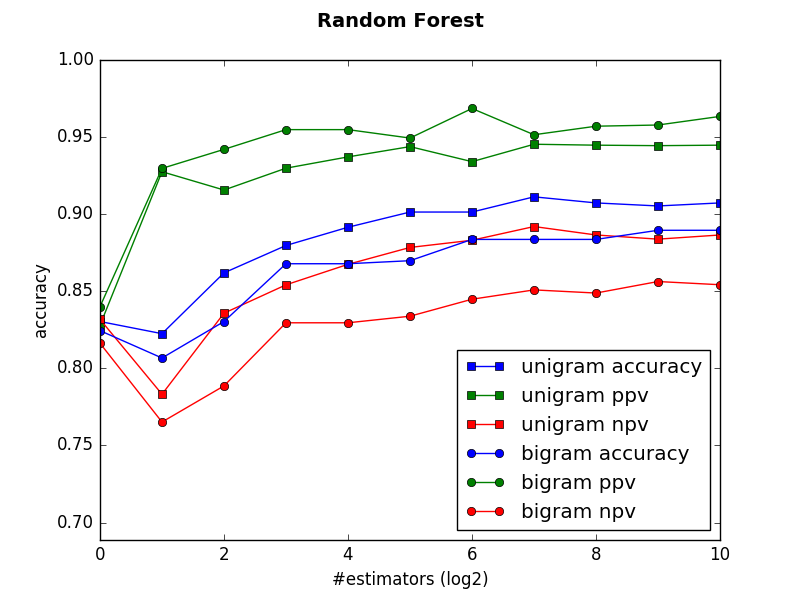
\includegraphics[width=\columnwidth]{../graphs/DisasterClassification/random_forest_unigram_vs_bigram_features.png}
	\caption{Disaster Classification Random Forest (Unigram vs. Bigram)}
	\label{fig:disaster_classification_rf}
\end{figure}

\begin{figure}[H]
	\centering
	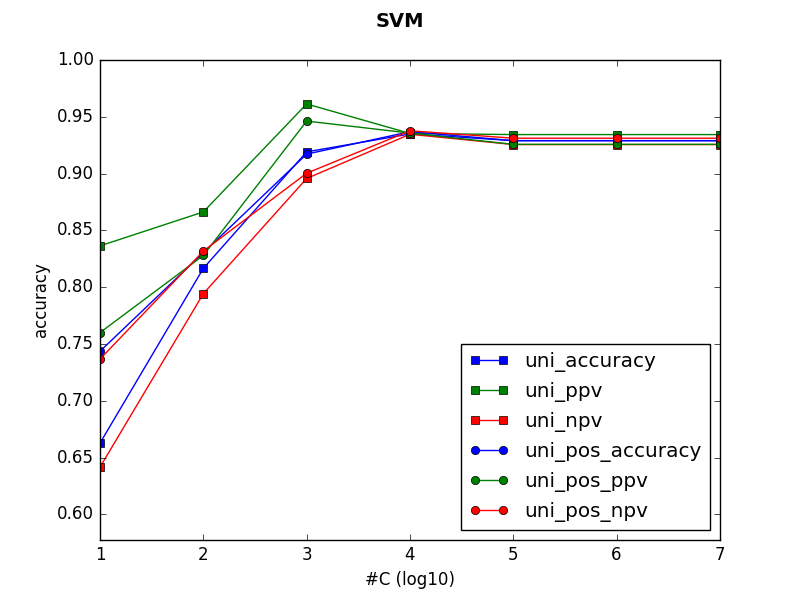
\includegraphics[width=\columnwidth]{../graphs/DisasterClassification/svm_uni_features.png}
	\caption{Disaster Classification SVM (Unigram vs. Unigram and POS)}
	\label{fig:disaster_classification_svm_uni}
\end{figure}

\begin{figure}[H]
	\centering
	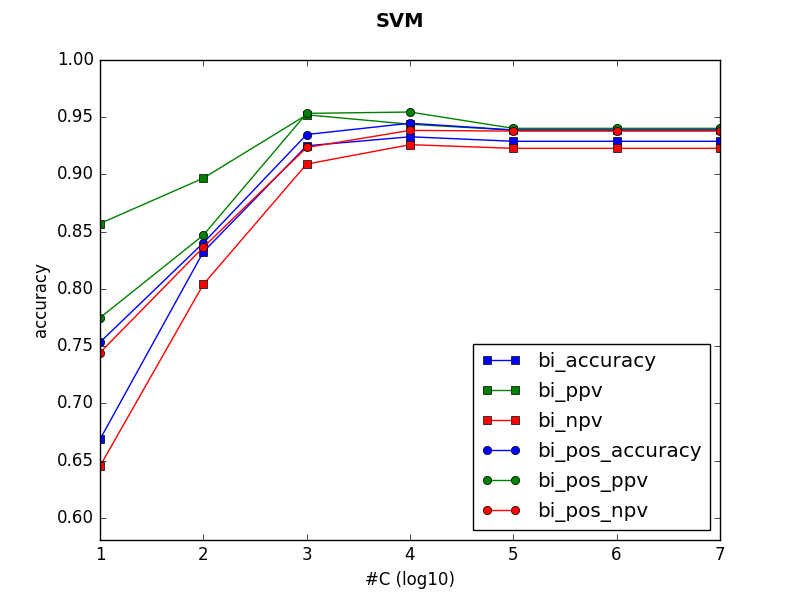
\includegraphics[width=\columnwidth]{../graphs/DisasterClassification/svm_bi_features.png}
	\caption{Disaster Classification SVM (Bigram vs. Bigram and POS)}
	\label{fig:disaster_classification_svm_bi}
\end{figure}

%%%%%%%%%%%%%%%%%%%%%%%%%%%%%%%%%%%%%%%%%%
\section{Sentiment Analysis of Tweets}

Sentiment analysis is considered to be a very interesting task in \textit{NLP}. It aims to determine the writer's attitude. Sentiment analysis tasks are usually target for multi-class classification such as feelings extraction (\textit{"sadness"}, \textit{"happiness"}, \textit{"anger"}, etc.). Another target may be classifying the \textit{polarity} of a given text (for example \textit{"positive"} or \textit{"negative"}). \\
We concentrated on the polarity task of classifying \textit{'disaster-related'} tweets as \textit{"objective"} or \textit{"subjective"}. In general vision, the ability of classifying \textit{'disaster-related'} tweets into these two categories may be used to extract facts and raise the confidence level of the disaster. \\
Although sentiment analysis is considered as a interesting task, it is surely a difficult one, combining it with tweets as dataset results an even more complicated task, since for the attributes we have spoken about in section 1.1. For example the following tweet is \textit{'disaster-related'}, but it is hard to tell whether it is objective or not:
\begin{center}
	\parbox{190pt}{\tweet{Thunder lightening torrential rain and a power cut!}}
\end{center}

\subsection{The Dataset}
Since supervised classification is requested, we needed a dataset containing labels of this polarity. However, we could not find any dataset \textit{'disaster related'} or not tweets with a \textit{objective/subjective} label. Therefore we extracted only \textit{'disaster related'} tweets from our original dataset (with confidence level $ \ge 0.9 $) and labeled them manually according to the following rule:
\begin{itemize}
	\item \textbf{Objective} is an undeniable truth. It is universally agreed upon. No logical person can deny that.
	\item \textbf{Subjective} is an opinion. The beauty is in the eye of the beholder.
\end{itemize}
We labeled 2,100 \textit{'disaster related'} tweets as \textit{objective/subjective} manually. Each tweet was labeled by two persons, on agreement, the label was kept, on disagreement, a third person broke the tie. Around 80\% of the tweets are objective while only 20\% are subjective.

\subsection{Feature Extraction}

We assumed that this task can achieve high accuracy without even using the words themselves (n-grams and meanings), but using the tweet structure, peripheral data and \textit{POS}-tagging. \\
To train the classifiers we extracted the following features for each tweet:

\begin{itemize}[noitemsep, nolistsep]
	\item Number of exclamation marks.
	\item Presence of exclamation mark.
	\item Number of question marks.
	\item Presence of question mark.
	\item Presence of \textit{URL}.
	\item Presence of emoticon (using \textit{emoticon.py} extractor from \textit{Twitter NLP} framework \cite{twitter_nlp}).
	\item Number of digits.
	\item Number of capital words.
	\item Number of capital letters.
	\item Number of punctuation marks and symbols (!"\#\$\%\&'()*+,-./:;<=>?@[\textbackslash]\^\_`\{\}\textasciitilde).
	\item Tweet's length.
	\item \textit{POS}-tagging:
		\begin{itemize}[noitemsep, nolistsep]
			\item Number of adjectives.
			\item Number of verbs.
			\item Number of adverbs.
			\item Number of pronouns.
			\item Number of proper nouns.
			\item Number of possessive endings.
		\end{itemize}
\end{itemize}

\subsection{Results}
We trained \textit{SVM} and \textit{Random Forest} classifiers for this job. Using $ C=10^4 $ as a penalty constant for \textit{SVM} and 128 estimators for \textit{Random Forest}.\\
Once again dataset was divide into train (90\%) and test (10\%) sets. Each classification method was tested with the previous mentioned features, using feature selection with \textit{ANOVA F-test} model. We repeated the test each time with more top $ K $ features selected by the feature selection model (out of 18 features total) and measured accuracies again. The goal was to find which features are the most important for our task. Measurements are total accuracy, \textit{PPV} and \textit{NPV}.\\

\paragraph{Random Forest} For the \textit{Random Forest} results \ref{fig:obj_sub_classification_rf}, we can see that best total accuracy is achieved with 13 features, so for \textit{NPV}, but best \textit{PPV} is achieved with only 1 feature (might be because of the biased dataset). The most influence features which were used are:
number of exclamation marks, presence of exclamation mark , presence of question mark, presence of URL, presence of emoticon, number of digits, number of capital letters, number of punctuation marks and symbols, tweeter's length.

\paragraph{SVM} For the \textit{Random Forest} results \ref{fig:obj_sub_classification_svm}, we can see that best total accuracy is achieved with 4 features only, so for \textit{NPV}, but best \textit{PPV} is achieved with only 1 feature as well (again, might be because of the biased dataset). The most influence features which were used are:
number of exclamation marks, presence of URL, presence of emoticon, number of punctuation marks and symbols.

The following tables \ref{tab:obj_sub_classifiaction_best_results} presents the best measurement result for each classifier (number of features used can be seen in column title), best total accuracy result (87.1\%) is achieved with \textit{Random Forest} classifier using 13 features. \\

\begin{table}[H]
	\caption{Objective/Subjective Classification Best Results}
	\label{tab:obj_sub_classifiaction_best_results}
	\begin{center}
		\scalebox{0.8}{
			\begin{tabular}{c | c | c | c | c }
				& \textbf{RF (1)} & \textbf{RF (13)} & \textbf{SVM (1)} & \textbf{SVM (4)} \\ \hline
				accuracy & 0.805 & 0.871 & 0.805 & 0.848 \\
				ppv & 0.905 & 0.890 & 0.905 & 0.874 \\
				npv & 0.500 & 0.750 & 0.500 & 0.667 \\
			\end{tabular}
		}
	\end{center}
\end{table}

\begin{figure}[H]
	\centering
	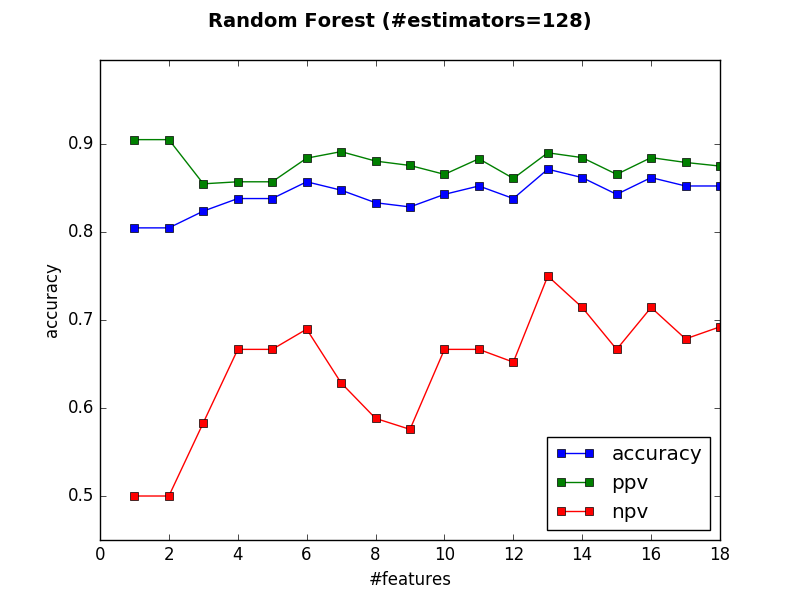
\includegraphics[width=\columnwidth]{../graphs/SentimentAnalysis/random_forest.png}
	\caption{Objective/Subjective Classification Random Forest}
	\label{fig:obj_sub_classification_rf}
\end{figure}

\begin{figure}[H]
	\centering
	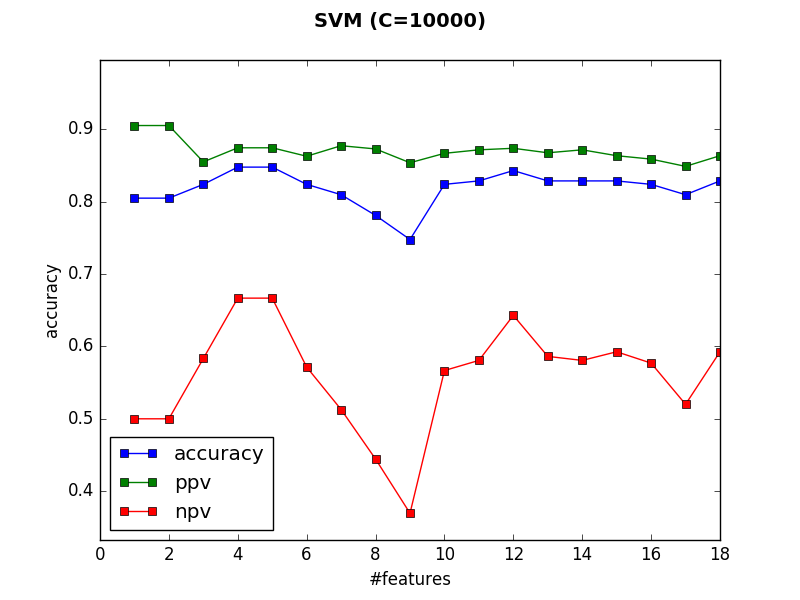
\includegraphics[width=\columnwidth]{../graphs/SentimentAnalysis/SVM.png}
	\caption{Objective/Subjective SVM}
	\label{fig:obj_sub_classification_svm}
\end{figure}

%%%%%%%%%%%%%%%%%%%%%%%%%%%%%%%%%%%%%%%%%%
\section{Named-Entity Recognition in Tweets}

In order to extract relevant information from disaster tweets, we have decided to use named entity recognition methods. NER allows us to classify people, organizations, locations and time expressions, which we can combine with our previous results for exposing relevant information on disasters.

\paragraph{GMB}\endnote{\textbf{"Groningen Meaning Bank" Dataset by University of Groningen}: comprises thousands of texts in raw and tokenised format, tags for part of speech, named entities and lexical categories, and discourse representation structures compatible with first-order logic. \url{http://gmb.let.rug.nl/}} In order to use NER, we used the Groningen Meaning Bank - a large corpus, composed of thousands of texts in raw and tokenized format, tags for part of speech, named entities and lexical categories, and discourse representation structures compatible with first-order logic. The top level categories of the corpus are:
\begin{itemize}[noitemsep, nolistsep]
	\item geo - Geographical Entity
	\item org - Organization
	\item per - Person
	\item gpe - Geopolitical Entity
	\item tim - Time indicator
	\item art - Artifact
	\item eve - Event
	\item nat - Natural Phenomenon
\end{itemize}
We used only the top categories, since they are sufficient for extracting relevant information on disasters from the tweets. The tags of the GMB corpus are translated to a NLTK compatible format, for using it combined with our previous results.

For tagging the named entities, a classifier based tagger can be used. We chose, for this part, the standard NLTK classifier. The best features of the tagger are unigrams, part of speech tagging, stemmer lemma of the current word, same attributes of the previous and next words, the previous tagging, and whether the current word is capitalized or contains special characters.

Tweets are often disorganized and does not contain structured sentences. In order to reduce errors, each tweet is treated as non-capitalized, and is stripped of URLs and special characters.

\paragraph{Results}

Three main categories of the GMB corpus remained relevant in the Tweeter world - location, organization, and geopolitical entity. A fourth category, time, was somewhat ambiguous - as it described both time entities and irrelevant ones. Other categories did not manage to reach any level of internal agreement on any entity.

By using the GMB corpus as the training data, we performed named entity recognition on the previously used dataset, of 10,877 labeled tweets. From those tweets, we singled out only those who were labeled as disasters. The main results were:

\begin{itemize}[noitemsep, nolistsep]
	\item Geographical Entity - California and Hiroshima were the dominant entities, as there were tweets about disasters in those places, followed by Japan, India, south, and Saudi Arabia.
	\item Organization - This category was composed by news companies, such as ABC, and by examples such as Obama, which was involved in the California disaster. Many user references are marked as an organization as well.
	\item Geopolitical Entity - Composed mostly of user references, and nationalities - Israeli, Turkish and much more.
	\item Time Indicator - ranged from a description of the current time - wildfire or typhoon, to description of the 70th anniversary of Hiroshima atom bombing.
\end{itemize}
From those results, we can learn the location, nationality of involvement, associated organizations, and  the type of the disaster.

%%%%%%%%%%%%%%%%%%%%%%%%%%%%%%%%%%%%%%%%%%
\section{Experimenting with Recent Tweets}

\todo{(Gal) Complete this section}
\paragraph{keywords}Twitter's Search API

% Omri's named entities on Chicago. Gal - you can compare them.

%geo Counter({'5000': 9, '8000': 9, 'los': 6, 'houston': 3, 'redlands-beaumont': 3, 'spousal': 2, 'europe': 2, 'russian': 2, 'spain': 2, 'burbank': 2, 'calumet': 1, 'london': 1, 'bionic': 1, 'steven': 1, 'snyders': 1, 'arkansas': 1, 'mexicos': 1, 'mueller': 1, 'california': 1, 'america': 1, 'semi': 1, 'augusta': 1, 'trumps': 1, 'ohio': 1, 'montreal': 1})
%org Counter({'userref': 18, 'la': 13, 'white': 5, 'los': 5, 'hammond': 4, 'chicago-firecom': 2, '55nb': 2, 'ib': 2, 'red': 2, 'chicago': 2, 'kirk': 2, 'csnchicagocom': 2, 'damn': 2, '2018': 2, 'fire': 2, '3-year-old': 2, 'hottimeinoldtowncom': 2, '5000 acres': 2, 'frankfurt': 2, 'burma': 1, 'uic': 1, 'brave': 1, 'deaddo': 1, 'herbo': 1, 'cbs': 1, 'mlssoccercom': 1, 'shelley': 1, 'bullsand': 1, 'fake': 1, 'blonde': 1, 'wan': 1, 'dexter': 1, 'rw': 1, 'foxsportscom': 1, 'archer': 1, 'harvey': 1, 'bathroom-break': 1, 'abc': 1, 'cleanup': 1, '3200-acre': 1, 'kankakee': 1, 'clarkgeothe': 1, 'match': 1, 'venezuela': 1, 'fast-moving': 1, 'springfield': 1, 'dad': 1, 'k-indemand': 1, 'nilsson': 1, 'california is on fire literally': 1, '1-comey': 1, 'update': 1, 'real-life': 1, 'california': 1, 'cubs': 1, 'icymi': 1, "'' national": 1, 'post-match': 1, 'bastian': 1, 'nra': 1, 'pilot': 1, '3000-acre': 1, 'alex': 1, 'peeve': 1, 'dream': 1, 'runway': 1, 'turkish': 1, 'twin': 1, 'mls': 1, 'american': 1, 'brooklyn': 1, 'mercedes': 1, 'wow': 1, 'black': 1})
%per Counter({'``': 1, 'richard': 1})
%gpe Counter({'gt': 1, 'chicago': 1, 'aww': 1, 'french': 1, 'userref': 1, 'italian': 1})
%tim Counter({'twitter ``': 19, 'angeles': 11, 'mls': 10, 'la history 10': 9, 'inland': 8, 'los angeles-area brush': 8, 'chicago': 6, 'twitter': 6, 'houston kechi': 5, 'fanly': 5, '1-0': 5, '7com la tuna': 5, 'austin chicago sun-times': 4, 'heroes': 4, 'spotify': 4, 'twitter `` los angeles': 4, 'fast-paced battle': 4, 'emblem': 4, 'hammond': 4, 'fire': 4, 'ants alligators lurking': 4, 'motorcycle-car collision in': 4, 'la history 10 percent': 4, '- chicago': 3, '1 chicago': 3, '-': 3, 'midway 5k': 3, 'here gt dept database info real coupons': 3, 'heroes - quick': 3, 'american flag': 3, 'st charles 1 chicago': 3, 'burbank': 3, 'st charles 1 chicago news': 3, 'burma': 3, 'search - 1chicagoorg two': 2, 'gtgt montreal impact 0 chicago fire': 2, 'bakes san': 2, 'history -': 2, 'few': 2, "'' please tune": 2, 'abc spain': 2, 'airplane': 2, '- when': 2, 'agt video 1390iheartcom plane': 2, 'denver': 2, 'soccer': 2, 'again -': 2, 'therapy': 2, 'agt video': 2, 'joe maddons muscle car': 2, 'twitter `` child': 2, 'twitter `` hammond pedestrian': 2, 'gon': 2, '73000 in': 2, 'teacher - tomonews - youtube': 2, 'gtgt match': 2, 'guy': 2, 'soundcloud': 2, 'twitter `` la tuna': 2, 'francisco - nbc': 2, '7com 3200-acre fire': 2, 'overnight': 2, 'nofilter sunset': 2, 'la tuna fire': 2, 'fire - boomerang': 2, 'dj frankie french': 2, 'london': 2, 'history - cnn': 2, '500 acres 7com 3200-acre fire': 2, '294 - fully': 2, 'august': 2, 'twitter `` schweinsteiger': 2, 'sound': 2, '`` playin': 2, 'urban outfitters': 2, 'four-game losing streak': 2, 'lauren': 2, 'userref userref': 2, 'madrid': 2, 'here 3y6kbcqzvb info': 2, 'mix 2 by': 2, "''": 2, 'e-mails': 2, 'twitter `` in': 2, 'cycle-car collision in': 2, 'twitter `` missing': 2, 'montreal red card': 2, 'august 10 2017 88zrcuiny 37lovpv': 1, 'montreal impact vs chicago fire': 1, 'shootings - nbc': 1, '271 truck 6 squad 1': 1, 'mo airport': 1, 'lee - before': 1, 'twitter `` i dont wan na': 1, '51kqst': 1, '70s amp 80s': 1, 'timecom dave tambellini': 1, 'muthafuckin': 1, 'nick jonas': 1, 'schweinsteiger': 1, 'lumineers': 1, 'street 4': 1, 'cf97 3ivwckr5q': 1, 'again rohingyagenocide rohingyamuslims': 1, 'agt video wgrb-am 1390iheartcom plane': 1, 'twitter `` terrifying footage': 1, 'porch 2k9wmgkyk4 7sgisf': 1, 'dodges': 1, 'harry nilsson': 1, 'arizona diamondbacks': 1, 'past': 1, 'earth': 1, 'nbc': 1, '975 on': 1, '- 2018 kia soul': 1, 'river search-and': 1, "`` work '' via": 1, 'these eclipses 8qk': 1, 'friend -': 1, '5000': 1, 'userref tim mcgill': 1, '98 -': 1, 'twitter `` 10': 1, 'la tuna canyon 7com man': 1, 'teacher': 1, '1 pm chicago': 1, '38': 1, 'bears userref': 1, 'cermakcanal chicagoscanner 7r2whtxj': 1, 'please buff': 1, 'store 4': 1, 'september 2 2017 chicagovideo 6xsmknlwwm': 1, 'via': 1, '-full blast- garage': 1, '24-0': 1, 'duck': 1, 'hot car': 1, 'high heels 7h9ocaorfw': 1, 'packaging - daniels': 1, 'userref stayinformed': 1, 'everybody': 1, 'usa': 1, 'leap toward': 1, 'oct not1more': 1, 'mind 96cbslocalcom dad sits': 1, 'hammond 2tvj0asqle 9ahdwt7rlw': 1, 'moro': 1, "famous '' ''": 1, 'cuts 8wzsqk6qzt': 1, '``': 1, 'floodwaters - cnn': 1, 'hillarys': 1, 'sept 1st even': 1, '4lut1m 1b': 1, 'impact chifire 2 15tu5o': 1, 'mumbai via': 1, 'snorkyjr': 1, 'king nathan vi': 1, 'twitter `` la': 1, '2017-09-03 josephking': 1, 'girls userref mv sales': 1, '1995': 1, 'cheapest': 1, 'roof': 1, '90s eerily': 1, 'here bradford doolittle': 1, 'trump': 1, 'candlelight vigil happening before': 1, 'my mutuals nerves 7pojdcl7': 1, 'la history 10 - 1chicagoorg la tuna': 1, 'espn fc chi fire': 1, 'fire 1huhy0pk': 1, 'kashmiri toddler 5yearold': 1, 'twitter `` match': 1, 'fr': 1, '1-0 win': 1, 'fannie mae': 1, 'espn fc chifire 2vij4c 9xvtiwy7nz': 1, 'berman stand-up comic who': 1, 'wed 1252': 1, 'la history noon chicago': 1, 'mazda cx-3': 1, 'plane': 1, 'mumbai 33': 1, 'eerie blinking': 1, 'area 7com 3200-acre fire': 1, 'frankfurt - autoblog jerome seaberg': 1, 'thing th': 1, 'baja california peninsula': 1, '6th': 1, 'gtgt polster': 1, 'alt360 -': 1, 'fireplace everyones': 1, 'houston': 1, 'la history 4truhbm': 1, 'hammond 1 chicago': 1, 'hammond chicago sun-times sun-times': 1, 'free-riding': 1, 'search - 1chicagoorg pedestrian fatally': 1, '5000 acres 10': 1, '46e56lgytw 60': 1, 'collision 9o dangerous': 1, 'kia soul': 1, '2012': 1, '- post-tribune everydayinchicago': 1, 'cf97 6rtwta': 1, 'video 9vjwkdfamv': 1, 'cf97 3wi8j 3pxzup5t': 1, 'hi rise': 1, 'friday night chicago news hammond': 1, 'foot': 1, 'hammond 1 chicago news': 1, 'impact chicago-fire match': 1, 'autonews carnews 0owpelwbz 9wpikdtvtp': 1, '18 usc 4 misprision re flynn false': 1, 'sept 7': 1, 'twitter `` sirslaysalot everybody': 1, '- chicago tribune chicagobreaking': 1, 'twitter `` here': 1, 'day -': 1, 'texas amp handling n ko': 1, 'chicago 15k more': 1, '58-year-old hammond': 1, 'our': 1, 'louisiana -': 1, 'wildfire destroys 5000 acres': 1, '2 sty ord 25x50 fire': 1, 'los angeles cbc': 1, 'til 6pm thank god everyone': 1, 'wrkf w adams 95': 1, '500 ourseason 8xarht1d6c': 1, 'twin peaks': 1, 'ass': 1, 'twitter `` today': 1, 'chance 1ji 0807f9d': 1, 'sound cloud np': 1, 'friday': 1, 'maybe 3 min': 1, 'quick': 1, 'california': 1, 'sierra nevada dream chaser space plane': 1, 'la history 10 percentcontained 5890uu4ey': 1, 'replacement - oops backdoor wont': 1, 'chicago 4pm': 1, 'shootings - nbc chicago chicago chicago': 1, 'twitter `` ft': 1, 'august 10 2017 gun': 1, 'nycs tribeca neighborhood': 1, 'fire 0p': 1, '1ssmjtzgtg': 1, '8vedk via metrouk 9bpbmsuf': 1, 'hair-raising': 1, 'impact - chicago tribune chicagosports': 1, 'midwest ah': 1, 'motorcycle-car collision in st': 1, 'sukin ampamp cum shot': 1, 'george': 1, 'hawaiian shirt': 1, 'impact 0sre8envb 8ngp8gmel': 1, 'dead landlord': 1, 'all 2o4wbx': 1, 'mama': 1, 'walking deadzombie apocalypse': 1, 'ants alligators lurking in': 1, 'userref': 1, 'smoke apocalypse sunsets 7ri2u9rdp': 1, 'july': 1, 'espn fc chi': 1, 'obama': 1, 'smoke apocalypse sunsets jad': 1, '15': 1, '19': 1, '1yuf7jqprc': 1, 'gresham porch chicago': 1, 'fire - nick da mind - youtube via': 1, 'montreal - cbc': 1, 'fire 14 muslim judges': 1, 'outburst straight outta compton': 1, 'twitter `` 2': 1, 'pct2017 dustin': 1, 'floodwaters - cnn video recruiter usa': 1, 'fedex kinkos i': 1, 'gotham': 1, 'season': 1, 'losing skid': 1, 'snipers': 1, 'here 3y6kbcqzvb info 76kjipyl0x': 1, 'past 10-man impact 1-0 - chicago': 1, 'here 5rss manyvids mvsales 13kxedvzd8': 1, 'twitter `` at joe maddons muscle car': 1, 'hammond pedestrian': 1, 'twitter `` blonde yoongi': 1, 'seasons': 1, 'rogers': 1, 'passengers 1slpp87qy 56ss2gse': 1, 'fire apparatus 73npo1unzl': 1, 'tech': 1, 'russia - aviation': 1, 'impact sept 2 2017': 1, 'scene leonardo dicaprio jonah hill -': 1, 'fundraiser': 1, 'detective': 1, '200 neo nazis and': 1, 'muthafuckin mcdonalds 0wpmu6jcz7': 1, 'austin chicago': 1, 'news 85xkv4': 1, 'chicago weekend': 1, 'latunafire 0mxmnfujqq': 1, 'brent ozar': 1, 'hitchhiker ampa corner': 1, 'impact': 1, 'chicago girl 13': 1, '9cqknxhkmd 9mjk': 1, 'jay': 1, 'nick da mind sacred': 1, 'twitter `` watch': 1, '5tpxcfh7': 1, 'september 1st yall': 1, 'montreal red card chicagofire 3dx7xf 9jtmg': 1, 'diamondbacks twins': 1, '4t332na36g': 1, '628 nialls ig story niall': 1, '42 usc': 1, 'pct2017 3aug19agmo': 1, 'teases concept': 1, 'twitter `` 38': 1, 'viral dog': 1, 'bar': 1, 'season chifire 4pjufwb': 1, 'nycs tribeca': 1, 'blue derkin': 1, 'landlord': 1, 'street 4o0t5uj5 3rgbln': 1, 'ib kennedy express': 1, 'guys chicago': 1, '0l6qg': 1, 'twitter `` dj foster': 1, 'season 5skurxqlxg thedansanto cf97': 1, "'' via nyt seven": 1, 'afghan': 1, 'mix 2 frankie': 1, 'mecca': 1, 'twittering': 1, 'harvey': 1, 'two-plus': 1, 'vinyl dj evil vince livevinyl on': 1, 'yoongi': 1, 'recently': 1, 'search - 1chicagoorg 2': 1, 'la history 7chicagocom la tuna': 1, 'cf97 section 8 chicago': 1, 'twitter `` father': 1, 'past 10-man impact 1-0 sep 02 2017': 1, 'twitter `` 1500-acre la tuna canyon': 1, 'vro': 1, '20 minutes 939myfmiheartcom utah': 1, 'la': 1, 'chicago ma chicago': 1, 'twitter `` dexter pottinger dead': 1, 'pre-show': 1, '92 -': 1, '7com evacuations': 1, '- post-tribune chicagobreaking': 1, 'userref -she': 1, 'userref fire': 1, 'twitter `` wan na': 1, 'three': 1, 'faraj': 1, 'twitter `` mercedes teases concept': 1, 'adri 22 on': 1, 'mike': 1, 'der komissar tune in': 1, '0zy': 1, 'florida dem election': 1, 'republicans': 1, 'twitter `` so': 1, '2nd alarm 340 n dearborn': 1, 'bull': 1, 'manyvids - hottest': 1, 'sochi russia plane dodges tornadoes in': 1, 'schweinsteiger lifts': 1, "`` 21st night of september ''": 1, 'padlocked svu': 1, 'mls 8jw10yy9c4 7s2c': 1, 'vs': 1, 'im': 1, 'userref from mom ``': 1, 'gtgt schweinsteiger': 1, '5000 acres': 1, 'userref playlist paper': 1, '- 1chicagoorg child': 1, 'news 5u5s6piv 7rnyr': 1, 'earth wind': 1, 'floodwaters 6k8pb38k 0l8khpu': 1, 'la burbank - la times': 1, '9elo': 1, 'anyone 1': 1, 'driver': 1, 'chicago scanner': 1, 'fame 0b3b9nj 5xrkefoq1': 1, 'night 7com la tuna': 1, 'twitter `` 20 games': 1, 'mil': 1, 'texas before depar': 1, '100 kilometer': 1, 'st ch': 1, 'over 3000 acres 7com la tuna': 1, 'tornadoes 60f2jvp 9rmi0vz': 1, '5000 acres 10 percent': 1, '10-man impact sbi': 1, '2 1 line': 1, 'fire apparatus 1com 10': 1, 'tirade': 1, 'upf40 cut 9': 1, 'charles -': 1, 'cemetery': 1, 'impact sept 2 2017 - youtube match': 1, 'ustream dj evil vince spins vinyl': 1, 'russia - youtube via': 1, '1 - 1chicagoorg child': 1, 'finder': 1, 'couple': 1, 'flooded 4': 1, 'abc7chicagocom abc 7 chicago': 1, 'twitter `` americans': 1, 'semi': 1, 'fire alisa alisa': 1, 'shes gon': 1, '2-comey': 1, 'monday nah': 1, 'unit req addl': 1, '750 acres 7com 3200-acre fire': 1, 'weekend shootings chicago 5p6wf6': 1, 'outburst page six via': 1, 'non-specification packaging': 1, 'hurricane': 1, '7sf 41ii96tvup': 1, 'sukin amp cum': 1, '9bvj7gmc': 1, 'twitter `` dangers': 1, 'innovation': 1, 'fat folks': 1, "'' via userref harvey updates": 1, 'bold': 1, 'photoshoot brooklyn beckham': 1, 'twitter `` justice department': 1, '8uboaa7 5hb9sz78l': 1, '13 yo science': 1, 'twitter `` ah russia': 1, 'weekend shootings 1 chicago news': 1, "'' -": 1, 'prompts 210 freeway closure 8i8dyl1cg': 1, 'al jazeera indian': 1, 'underway': 1, '975 radio hits': 1, 'saratoga horseracing': 1, 'daniels midland ceo dwayne andreas': 1, 'classic justin ori': 1, 'twitter `` chasethedawn': 1, 'gtgt': 1, 'userref polite fire': 1, 'werntz': 1, '3bop': 1, 'seeker': 1, 'suit': 1, "bon bini ''": 1, 'twitter `` chicago': 1, 'kerwynn williams rotoworld': 1, 'hawaiian': 1, 'france 38': 1, 'twitter `` peoplesoracle': 1, "'' album 1z5 44xyn82": 1, 'twitter `` update pedestrian': 1, 'thebiodome chicago illinois livevinyl': 1, 'mind 38rubmf cbsnews 4px4umn00': 1, 'history - cnn recruiter usa': 1, '- chicago tribune everydayinchicago': 1, 'age': 1, 'twitter `` sold': 1, 'moore': 1, 'classic': 1, '3335 bayan': 1, '1980s none': 1, 'passengers 6hvepshyhx': 1, 'about stuff': 1, 'userref cops chase pickup pickup driver': 1, 'yoga': 1, 'autonews carnews mercedes teases concept': 1, 'peters sphr': 1, 'userref maybe': 1, '5': 1, 'tower 2gddh 1wfepz2fkf': 1, 'everyone tho oliver': 1, '10': 1, 'los angeles': 1, 'september -': 1, 'tx-debarking plane- amp': 1, 'twitter `` dad sits': 1, '939 my': 1, 'blue oh m': 1, '7com man': 1, 'newser': 1, 'patio cool breeze skyline': 1, 'sun shade': 1, '- 1ceqlox': 1, 'impact sept 2': 1})
%art Counter({'rush': 2, 'whalum': 2, 'no': 2, 'costly': 1, 'these': 1, '``': 1, 'brandon': 1, 'fire': 1, 'treasury': 1, 'tan': 1})
%nat Counter({'how': 1, '``': 1, 'trump': 1})
%eve Counter({'writers': 1})


%%%%%%%%%%%%%%%%%%%%%%%%%%%%%%%%%%%%%%%%%%
\section{Conclusions}

\paragraph{Future work} TODO

%%%%%%%%%%%%%%%%%%%%%%%%%%%%%%%%%%%%%%%%%%

{\footnotesize \bibliographystyle{acm}
\bibliography{references}}

\theendnotes

\end{document}







